
Below, I describe the Scottish agriculture industry; beaver ecology, territorial expansion, and behavior, including potential threats to agricultural productivity; and the recent reemergence of beavers in Scotland. 

\subsection{Agriculture in Scotland}
Modern Scottish agriculture, built in a cool and marshy environment, has relied on an array of floodbanks constructed along rivers to protect cropland from inundation (\cite{goldfarb_eager_2018}). In 2023, 69\% (5.33 million hectares) of Scotland's land area was devoted to agricultural use \citep{cabinet_secretary_for_rural_affairs_land_reform_and_islands_results_2023}, with much of the arable farming concentrated along the eastern lowlands. The industry employs a 66,000-person workforce (about 1.2\% of the country's population), contributing approximately 2.5 billion euros of Standard Output.\footnote{A standard EU metric for measuring the economic weight of agricultural activity, standard output equals the average value of output (in euros) per hectare of farmland or per head of livestock.} 13\% of the agricultural workforce is concentrated in Tayside, which relies heavily on casual and seasonal employees. In 2016, Scotland's farm income was estimated at \pounds 667 million, roughly 18\% of the United Kingdom's total farm income. The majority of farms report a farm business income below \pounds 30,000, with 22\% operating at a loss. Most arable farming in Scotland is dedicated to above-ground cereals, including barley, oats, and rye, and to a lesser extent, crops such as oilseed rape and beans. In contrast to the rugged northwest highlands, where holdings are largely under five hectares, in the arable lowlands, where beavers reemerged, farm size is distributed evenly from less than one hectare to over 200 hectares. My 1km$^2$ (100 hectares) unit of analysis is informed by this distribution.

\subsection{Beavers}
\label{sec:background-beavers}
Beavers, including the North American \textit{Castor canadensis} and the Eurasian \textit{Castor fiber}, are large herbivorous rodents. Requiring water, they tend to settle on streams, rivers, lakes, or ponds, preferring areas with little to no gradient \citep{muller-schwarze_beaver_2011}, narrow watercourses \citep{dittbrenner_modeling_2018}, slow-moving water, and nearby vegetation \citep{swinnen_environmental_2019}. Constructed from timber, branches, mud, and leaves, beaver dams may stretch up to hundreds of meters and form ponds, often with several to a single colony (\cite{muller-schwarze_beaver_2011}). The family unit resides in a lodge, either burrowed into the river bank or built as a free-standing structure in the impounded water. The beaver often dredges a network of canals around the colony to facilitate movement between its lodge and feeding areas \citep{muller-schwarze_beaver_2011}. The typical litter has 3 or 4 kits, which spend around two years with their parents before departing to establish homes (\cite{hartman_notes_1997}, \cite{muller-schwarze_beaver_2011}), usually within 5 kilometers of the parents. Dispersal almost always occurs along the river, though temporary waterways formed during spring snowmelt can facilitate passage across otherwise inaccessible dry land. 

As a keystone species and ecosystem engineer, the beaver reforms its habitat. A large literature documents a host of positive externalities from beaver colonization. Species richness and biodiversity rise (\cite{hossack_trends_2015}, \cite{wright_ecosystem_2002}, \cite{leidholt-bruner_beaver_1992}, \cite{bouwes_ecosystem_2016}, \cite{fedyn_beyond_2023}, \cite{kemp_qualitative_2012}, \cite{stringer_impacts_2016}, \cite{law_habitat_2016}), climate extremes and pollution are mitigated via carbon storage and water filtration (\cite{hood_beaver_2008}, \cite{dewey_beaver_2022}, \cite{johnston_beaver_2014}, \cite{fairfax_using_2018}, \cite{fairfax_smokey_2020}, \cite{lazar_beaver_2015}, \cite{wohl_landscape-scale_2013}), and local economies see increased tourism revenue (e.g., \cite{campbell_economic_2007} and \cite{auster_wildlife_2020}).

But the beaver's consumption of natural resources, for construction materials and food, may conflict with human land use needs. Water impounded by beaver dams floods roads during periods of high precipitation and snow melt, particularly when beavers plug highway culverts \citep{jensen_habitat_2001}. Beavers may target vegetation on residential property, with many homeowners viewing beavers as a nuisance species that should be controlled \citep{jonker_experiences_2006}. Agriculture represents by far the largest economic concern related to beaver cohabitation (\cite{hamilton_tayside_2015}, \cite{noauthor_beavers_2017}, \cite{mikulka_european_2020}, \cite{janiszewski_damage_2019}, \cite{campbell-palmer_managing_2015}). Burrowing into river banks may collapse fields, dams impound moving water that may flood fields, beavers may graze on crops, and orchard trees may be felled for use as construction materials.

\subsubsection{Scottish Reemergence}

In 1996, the Scottish public conservancy began studying the feasibility of reintroducing the Eurasian beaver \citep{kitchener_history_1997}. Though present in the British Isles since at least 10,000 years ago, the beaver went extinct in Scotland sometime between the 12th and 16th Centuries, hunted for its pelt, meat, and prized \textit{castoreum} oil \citep{kitchener_history_1997}. Similar local extinctions and near-extinctions occurred throughout mainland Europe and North America in the 18th and 19th Centuries. Over the past century, beavers have repopulated, through both controlled release and natural expansion, much of their former range (\cite{dzieciolowski_reintroduction_1999}, \cite{janiszewski_restoration_2021}, \cite{schwab_beaver_2003}, \cite{hartman_patterns_1995}, \cite{dijkstra_reintroduction_1999}). Despite its status being of least concern, \textit{Castor fiber} is now listed as an Annex IV(a) species in the EU Habitats Directive\footnote{Article 12(1) of the Habitats Directive prohibits the killing and capture of Annex IV(a) species, as well as disturbance of their habitat \citep{noauthor_council_2013} Annex IV(a) protection does not apply to the populations of Finland, Sweden, Latvia, Lithuania, Estonia, and Poland, which are listed under the softer Annex V, allowing for management action to avoid over-exploitation.}. 

Around 2000, wild beavers emerged in Scotland, either released by an unauthorized entity, escaped from a nearby enclosure, or stowed-away on ships from mainland Europe (\textcolor{red}{cites}). While this population spread around the agriculturally productive lowland River Tay region (\ref{fig:study-area}), a controlled release occurred in Knapdale, on the rugged western coast of Scotland \citep{campbell-palmer_managing_2015}. In 2012, the national conservancy conducted the first regional survey of the Tayside beavers, followed by two others in 2017 and 2020, respectively. In 2016, despite fierce opposition from agricultural groups (\cite{castle_beavers_2021}, \cite{kennedy_nfu_2023}, \cite{werth_christopher_beavers_2017}), the Scottish government, citing the EU Habitats Directive, allowed the Tayside population to remain (\textcolor{red}{cite govt policy statement}). In 2019, beavers became a protected species \citep{noauthor_beavers_2019}. While official policy encourages non-lethal mitigation measures, hundreds of beavers have been culled since obtaining protected status, with 202 individuals killed between 2019 and 2021, not including unauthorized killing undertaken by private landowners \citep{williams_more_2021}. 

The fear of conflict between beavers and agricultural operations is not unfounded. For example, during the expansion of beaver populations in Bavaria in the 20th Century, the landscape of intensive agriculture, supported by a network of engineered waterways--similar to the eastern Scottish lowlands--saw large-scale disruption \citep{campbell-palmer_managing_2015}. By the 1990s, several farmers organizations were advocating for the extirpation of beavers from the region. In Scotland, official estimates of beaver-caused damage are scarce. To my knowledge, \cite{hamilton_tayside_2015} is the only study of the Scottish beaver's economic impact. In contrast to this paper's ex-post analysis of realized land use changes, the authors project potential impacts by scaling up landowner-reported costs, estimating a total cost of 179,900 GBP for the Tayside region, almost all of which (173,500 GBP) is incurred in the agriculture-intensive eastern lowlands. The majority of reported costs come from labor costs to process and replace of felled trees and repair flood banks. Compared to bank, crop, and tree damage, survey respondents rarely cited field flooding as the primary damage.

\begin{figure}
    \centering
    \caption{Study region}
    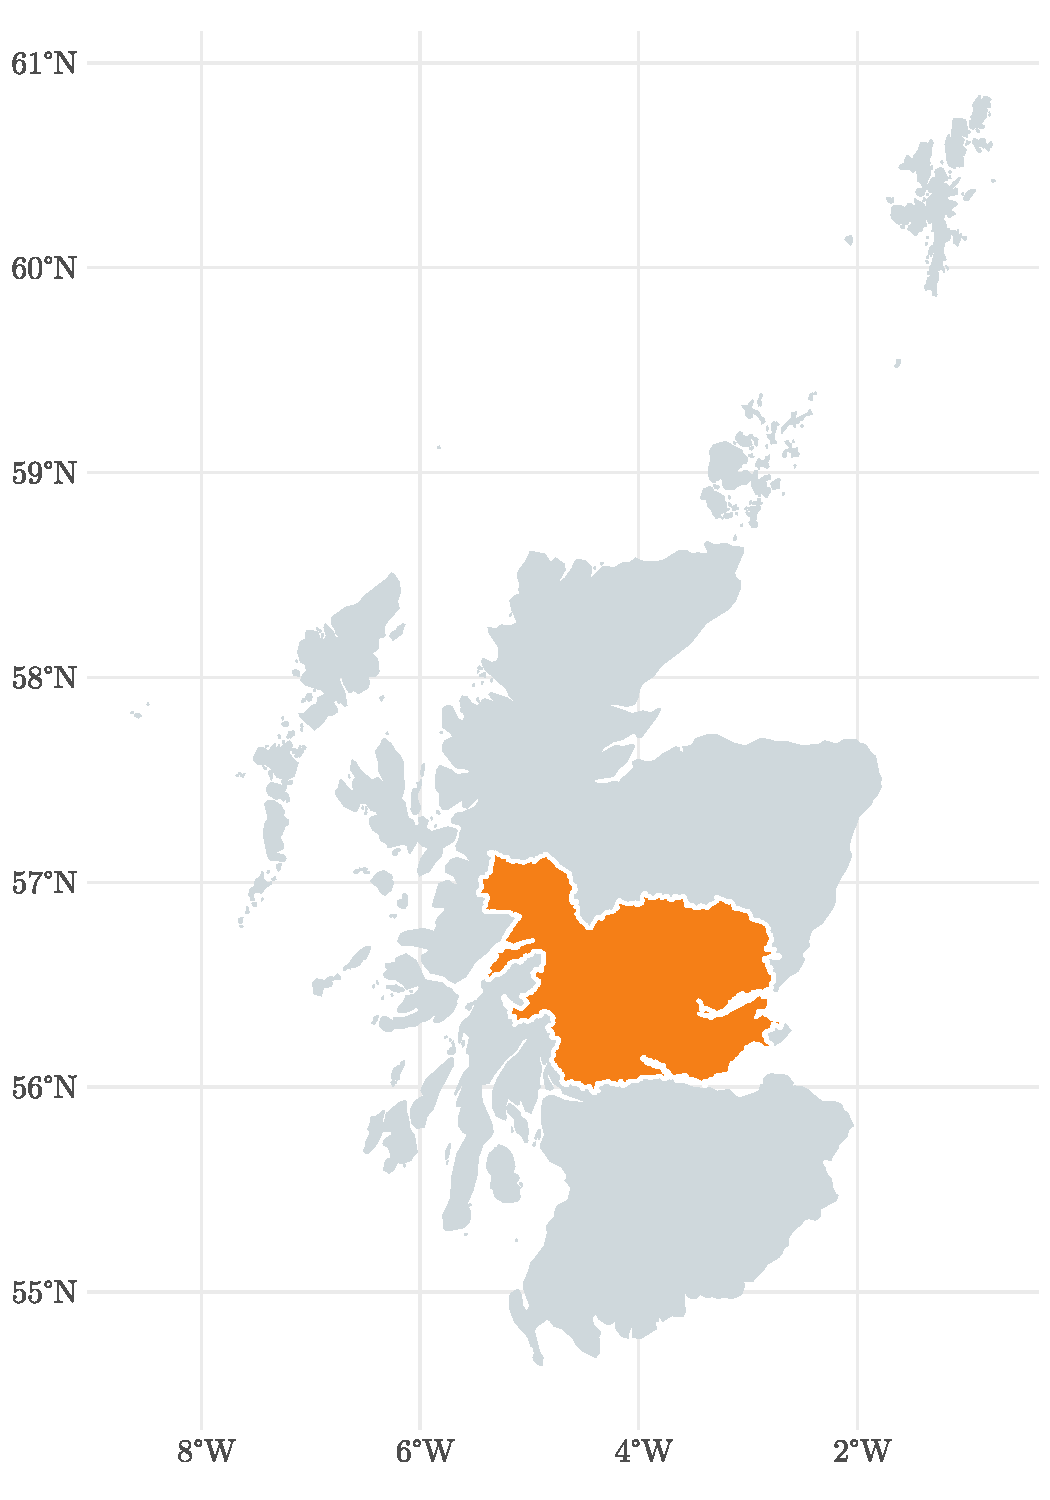
\includegraphics[width=0.4\linewidth]{output/figures/study_area.pdf}
    \label{fig:study-area}
    \caption*{\justifying \footnotesize Notes: Study region within Scotland (orange), capturing a buffer area around beaver expansion in the Tay, Earn, South Esk, Lunan, and Perth Coastal catchments. Agricultural parish boundaries are drawn in gray.}
\end{figure}